\documentclass[conference]{IEEEtran}
\usepackage[T1]{fontenc}
\usepackage{lmodern}
\usepackage[utf8]{inputenc}
\usepackage{newtxtext}
\usepackage{tikz}
\usetikzlibrary{positioning,arrows.meta,shapes.multipart,fit,calc,shapes.geometric,shapes,shapes.symbols,arrows}
\usepackage{tabularx}
\usepackage{booktabs}
\usepackage{siunitx}
\sisetup{round-mode=places, round-precision=2}
\usepackage{array}
\usepackage{graphicx}
\usepackage{amsmath}
\usepackage{amssymb}
\usepackage{pifont}
\newcommand{\cmark}{\ding{51}}
\newcommand{\xmark}{\ding{55}}
\usepackage{url}
\usepackage[backend=biber]{biblatex}
\addbibresource{reference.bib}
\addbibresource{demo_refs.bib}
\renewcommand{\textfraction}{0.05}
\renewcommand{\floatpagefraction}{0.8}

\begin{document}

\title{VTTSI-Chat: Real-Time Intersection Safety Monitoring\\
with LLM-Powered Natural Language Explanation}

\author{
\IEEEauthorblockN{Cheng-Shun Chuang}
\IEEEauthorblockA{\textit{Computer Science}\\
Virginia Tech, Alexandria, VA\\
cchengshun@vt.edu}
\and
\IEEEauthorblockN{Jason Cusati}
\IEEEauthorblockA{\textit{Computer Science}\\
Virginia Tech, Blacksburg, VA\\
djjay@vt.edu}
\and
\IEEEauthorblockN{Victory Uhunmwangho}
\IEEEauthorblockA{\textit{Computer Science}\\
Virginia Tech, Blacksburg, VA\\
victoryu@vt.edu}
}

\maketitle

\sloppy
\raggedbottom

\begin{abstract}
We present \textbf{VTTSI-Chat}, a cloud-native system that pairs the Virginia Tech
Transportation Safety Index (VTTSI)---a hybrid Real-Time Safety Index (RT--SI) and
CRITIC-weighted MCDM pipeline---with a \textbf{SafetyChat} conversational module
powered by a tool-augmented GPT-4o.
VTTSI fuses seven years of VDOT crash records via Empirical Bayes stabilization with
live connected-vehicle telemetry, producing interpretable 0--100 safety scores every
15 minutes.
SafetyChat exposes six typed API tools to the LLM, grounding all natural language
responses in live data and enabling TMC operators, planners, and emergency responders
to query causal safety narratives through ordinary conversation.
A live deployment at
\url{https://cs6604-trafficsafety-180117512369.europe-west1.run.app}
demonstrates four end-to-end use cases across monitored intersections in Falls Church, VA.
\end{abstract}

% ─────────────────────────────────────────────────────────
\section{Introduction}
\label{sec:intro}

TMC operators must interpret multi-dimensional safety indices under time pressure, yet
existing dashboards present data without explaining causality or suggesting actions.
Tool-augmented LLMs can reason over structured numerical data to produce grounded
explanations \cite{toolformer2023}, but prior LLM+traffic work targets signal control
\cite{llmlight2024} or AV motion planning \cite{gptdriver2023,drivevlm2024}---not
safety-index explanation for infrastructure operators.

\textbf{VTTSI-Chat} closes this gap by pairing the VTTSI hybrid scoring pipeline with
\textbf{SafetyChat}: a GPT-4o module that issues typed function calls to live VTTSI
endpoints and returns causal safety narratives via natural language dialogue.
It is the first system to combine a hybrid EB-stabilized crash index with real-time
MCDM scoring \emph{and} an operator-facing LLM explanation layer.

% ─────────────────────────────────────────────────────────
\section{VTTSI System Overview}
\label{sec:system}

\begin{figure*}[t]
\centering
\resizebox{\textwidth}{!}{%
% ============================================================
%  VTTSI Refined System Architecture (Vite Dashboard with SafetyChat)
%  Usage: % ============================================================
%  VTTSI Refined System Architecture (Vite Dashboard with SafetyChat)
%  Usage: % ============================================================
%  VTTSI Refined System Architecture (Vite Dashboard with SafetyChat)
%  Usage: \input{system-architecture} inside a figure* environment
% ============================================================
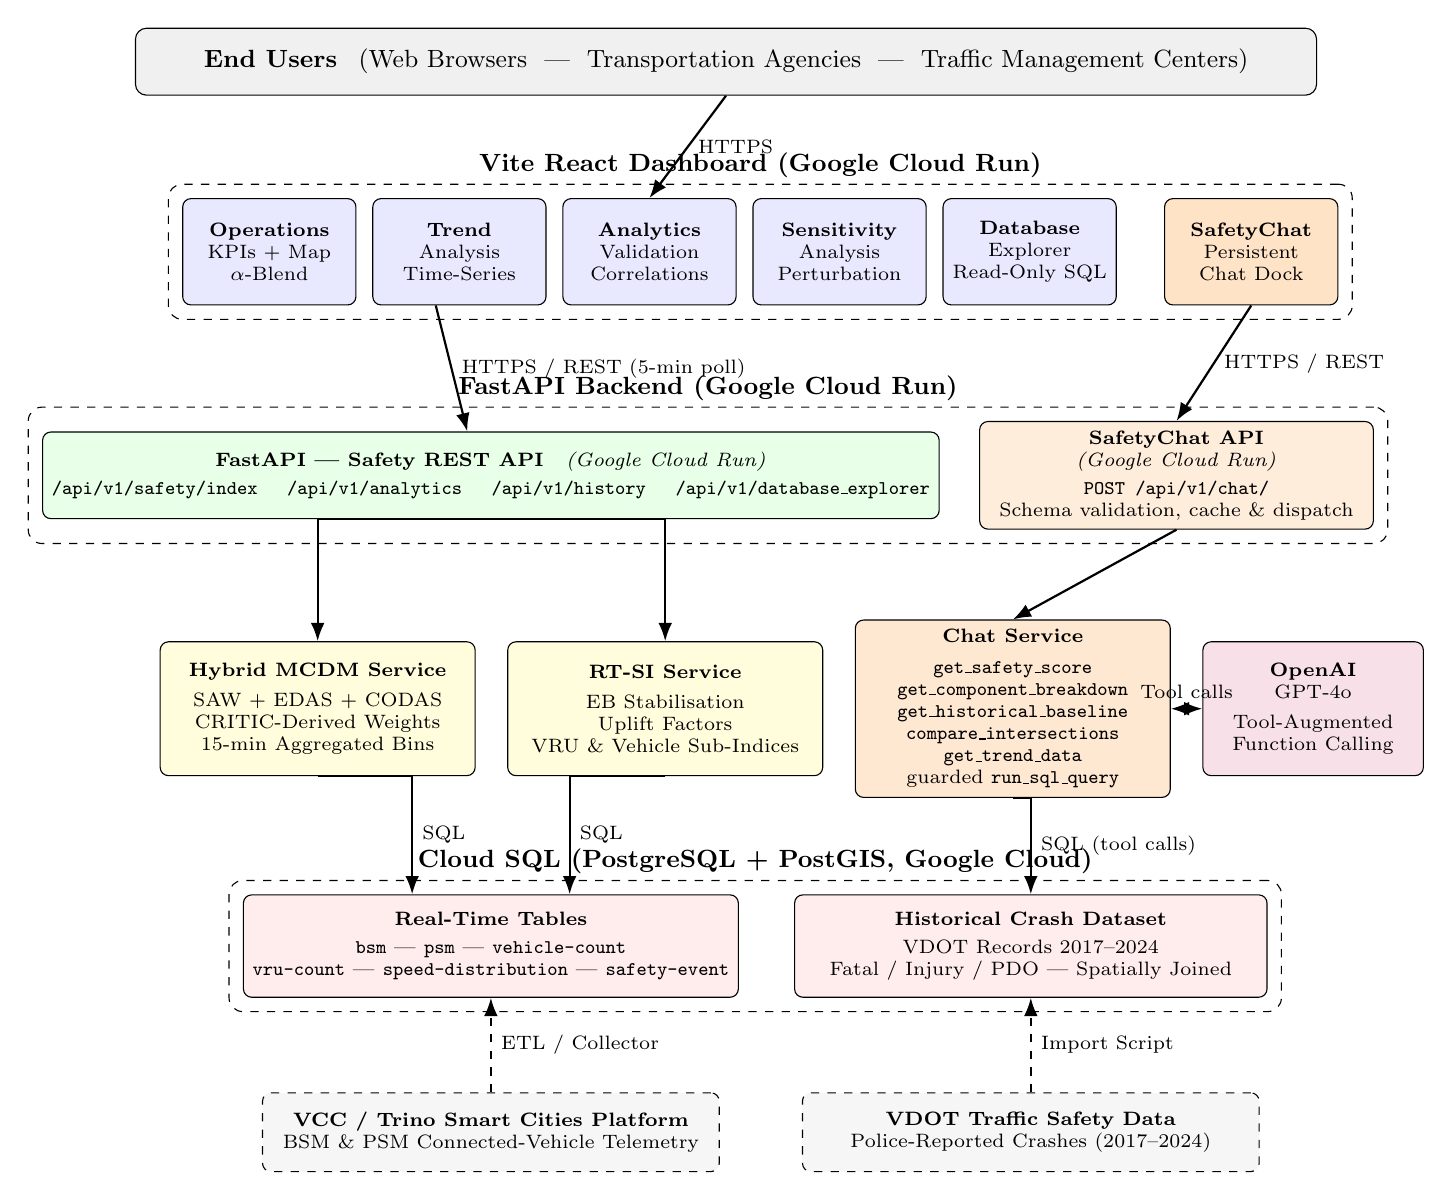
\begin{tikzpicture}[
    >=Latex,
    font=\small,
    % ── node styles ──────────────────────────────────────────
    user/.style    ={rectangle, draw, rounded corners=4pt, fill=gray!12,
                     minimum width=15cm, minimum height=0.85cm, align=center},
    page/.style    ={rectangle, draw, rounded corners=3pt, fill=blue!9,
                     minimum width=2.2cm, minimum height=1.35cm,
                     align=center, font=\scriptsize},
    chatpage/.style={rectangle, draw, rounded corners=3pt, fill=orange!22,
                     minimum width=2.2cm, minimum height=1.35cm,
                     align=center, font=\scriptsize},
    api/.style     ={rectangle, draw, rounded corners=3pt, fill=green!9,
                     minimum width=7.8cm, minimum height=1.1cm,
                     align=center, font=\scriptsize},
    chatapi/.style ={rectangle, draw, rounded corners=3pt, fill=orange!14,
                     minimum width=5.0cm, minimum height=1.1cm,
                     align=center, font=\scriptsize},
    svc/.style     ={rectangle, draw, rounded corners=3pt, fill=yellow!14,
                     minimum width=4.0cm, minimum height=1.7cm,
                     align=center, font=\scriptsize},
    chatsvc/.style ={rectangle, draw, rounded corners=3pt, fill=orange!18,
                     minimum width=4.0cm, minimum height=1.7cm,
                     align=center, font=\scriptsize},
    llm/.style     ={rectangle, draw, rounded corners=3pt, fill=purple!12,
                     minimum width=2.8cm, minimum height=1.7cm,
                     align=center, font=\scriptsize},
    dbtab/.style   ={rectangle, draw, rounded corners=3pt, fill=red!7,
                     minimum width=6.0cm, minimum height=1.3cm,
                     align=center, font=\scriptsize},
    ext/.style     ={rectangle, draw, dashed, rounded corners=3pt, fill=gray!7,
                     minimum width=5.8cm, minimum height=1.0cm,
                     align=center, font=\scriptsize},
    grpbox/.style  ={rectangle, draw, dashed, rounded corners=5pt, inner sep=5pt},
    arr/.style     ={->, thick, >=Latex},
    darr/.style    ={->, thick, dashed, >=Latex},
]

% ── TIER 0 : Users ────────────────────────────────────────────────────────────
\node[user] (user)
    {\textbf{End Users}
     \enspace(Web Browsers \ | \ Transportation Agencies \ | \
              Traffic Management Centers)};

% ── TIER 1 : Vite frontend dashboard panels ─────────────────────────────────
\node[page, below=1.3cm of user, xshift=-5.8cm] (p0)
    {\textbf{Operations}\\KPIs + Map\\$\alpha$-Blend};
\node[page, right=0.2cm of p0] (p1)
    {\textbf{Trend}\\Analysis\\Time-Series};
\node[page, right=0.2cm of p1] (p2)
    {\textbf{Analytics}\\Validation\\Correlations};
\node[page, right=0.2cm of p2] (p3)
    {\textbf{Sensitivity}\\Analysis\\Perturbation};
\node[page, right=0.2cm of p3] (p4)
    {\textbf{Database}\\Explorer\\Read-Only SQL};
\node[chatpage, right=0.6cm of p4] (p5)
    {\textbf{SafetyChat}\\Persistent\\Chat Dock};

\node[grpbox, fit=(p0)(p1)(p2)(p3)(p4)(p5),
      label={[font=\small\bfseries, fill=white, inner sep=2pt,
              rounded corners=2pt]above:{Vite React Dashboard (Google Cloud Run)}}]
      (fe_box) {};

% ── TIER 2 : Backend API layer ────────────────────────────────────────────────
% api_main placed so it roughly centres on analysis pages p0-p3
\node[api, below=1.6cm of p1, xshift=0.4cm] (api_main)
    {\textbf{FastAPI --- Safety REST API}\quad\textit{(Google Cloud Run)}\\[2pt]
     \texttt{/api/v1/safety/index} \quad
     \texttt{/api/v1/analytics} \quad
     \texttt{/api/v1/history} \quad
     \texttt{/api/v1/database\_explorer}};

\node[chatapi, right=0.5cm of api_main] (api_chat)
    {\textbf{SafetyChat API}\\
     \textit{(Google Cloud Run)}\\[2pt]
     \texttt{POST /api/v1/chat/}\\
     Schema validation, cache \& dispatch};

\node[grpbox, fit=(api_main)(api_chat),
      label={[font=\small\bfseries, fill=white, inner sep=2pt,
              rounded corners=2pt]above:{FastAPI Backend (Google Cloud Run)}}]
      (be_box) {};

% ── TIER 3 : Core services ────────────────────────────────────────────────────
\node[svc, below=1.55cm of api_main, xshift=-2.2cm] (mcdm)
    {\textbf{Hybrid MCDM Service}\\[3pt]
     SAW + EDAS + CODAS\\
     CRITIC-Derived Weights\\
     15-min Aggregated Bins};

\node[svc, right=0.4cm of mcdm] (rtsi)
    {\textbf{RT-SI Service}\\[3pt]
     EB Stabilisation\\
     Uplift Factors\\
     VRU \& Vehicle Sub-Indices};

\node[chatsvc, right=0.4cm of rtsi] (chatsvc)
    {\textbf{Chat Service}\\[3pt]
     \texttt{get\_safety\_score}\\
     \texttt{get\_component\_breakdown}\\
     \texttt{get\_historical\_baseline}\\
     \texttt{compare\_intersections}\\
     \texttt{get\_trend\_data}\\
     guarded \texttt{run\_sql\_query}};

\node[llm, right=0.4cm of chatsvc] (llm)
    {\textbf{OpenAI}\\GPT-4o\\[3pt]
     Tool-Augmented\\Function Calling};

% ── TIER 4 : Database ─────────────────────────────────────────────────────────
% db_rt centred roughly under mcdm+rtsi; db_crash under chatsvc
\node[dbtab, below=1.5cm of mcdm, xshift=2.2cm] (db_rt)
    {\textbf{Real-Time Tables}\\[2pt]
     \texttt{bsm} | \texttt{psm} | \texttt{vehicle-count}\\
     \texttt{vru-count} | \texttt{speed-distribution} | \texttt{safety-event}};

\node[dbtab, right=0.7cm of db_rt] (db_crash)
    {\textbf{Historical Crash Dataset}\\[2pt]
     VDOT Records 2017--2024\\
     Fatal / Injury / PDO --- Spatially Joined};

\node[grpbox, fit=(db_rt)(db_crash),
      label={[font=\small\bfseries, fill=white, inner sep=2pt,
              rounded corners=2pt]above:{Cloud SQL (PostgreSQL + PostGIS, Google Cloud)}}]
      (db_box) {};

% ── TIER 5 : External data sources ───────────────────────────────────────────
\node[ext, below=1.2cm of db_rt] (ext_vcc)
    {\textbf{VCC / Trino Smart Cities Platform}\\
     BSM \& PSM Connected-Vehicle Telemetry};

\node[ext, below=1.2cm of db_crash] (ext_vdot)
    {\textbf{VDOT Traffic Safety Data}\\
     Police-Reported Crashes (2017--2024)};

% ── ARROWS ────────────────────────────────────────────────────────────────────

% Users → Frontend (route to p2 node, centre of the analysis pages row)
\draw[arr] (user.south) -- node[right, font=\scriptsize]{HTTPS}
    (p2.north);

% Frontend analysis pages → Safety API (route straight into api_main)
\draw[arr] ([xshift=-0.3cm]p1.south) --
    node[right, font=\scriptsize]{HTTPS / REST (5-min poll)}
    ([xshift=-0.3cm]api_main.north);

% SafetyChat page → Chat API
\draw[arr] (p5.south) -- node[right, font=\scriptsize]{HTTPS / REST}
    (api_chat.north);

% Safety API → MCDM & RT-SI services
\draw[arr] (api_main.south) -| (mcdm.north);
\draw[arr] (api_main.south) -| (rtsi.north);

% Chat API → Chat Service
\draw[arr] (api_chat.south) -- (chatsvc.north);

% Chat Service <-> OpenAI (bidirectional)
\draw[<->, thick] (chatsvc.east) --
    node[above, font=\scriptsize]{Tool calls}
    (llm.west);

% MCDM → Real-Time DB
\draw[arr] (mcdm.south) -|
    node[pos=0.75, right, font=\scriptsize]{SQL}
    ([xshift=-1.0cm]db_rt.north);

% RT-SI → Historical DB
\draw[arr] (rtsi.south) -|
    node[pos=0.75, right, font=\scriptsize]{SQL}
    ([xshift=1.0cm]db_rt.north);

% Chat Service → Historical DB (LLM tool queries)
\draw[arr] (chatsvc.south) -|
    node[pos=0.75, right, font=\scriptsize]{SQL (tool calls)}
    (db_crash.north);

% External sources → DB (ETL ingestion, dashed)
\draw[darr] (ext_vcc.north) --
    node[right, font=\scriptsize]{ETL / Collector}
    (db_rt.south);
\draw[darr] (ext_vdot.north) --
    node[right, font=\scriptsize]{Import Script}
    (db_crash.south);

\end{tikzpicture}
 inside a figure* environment
% ============================================================
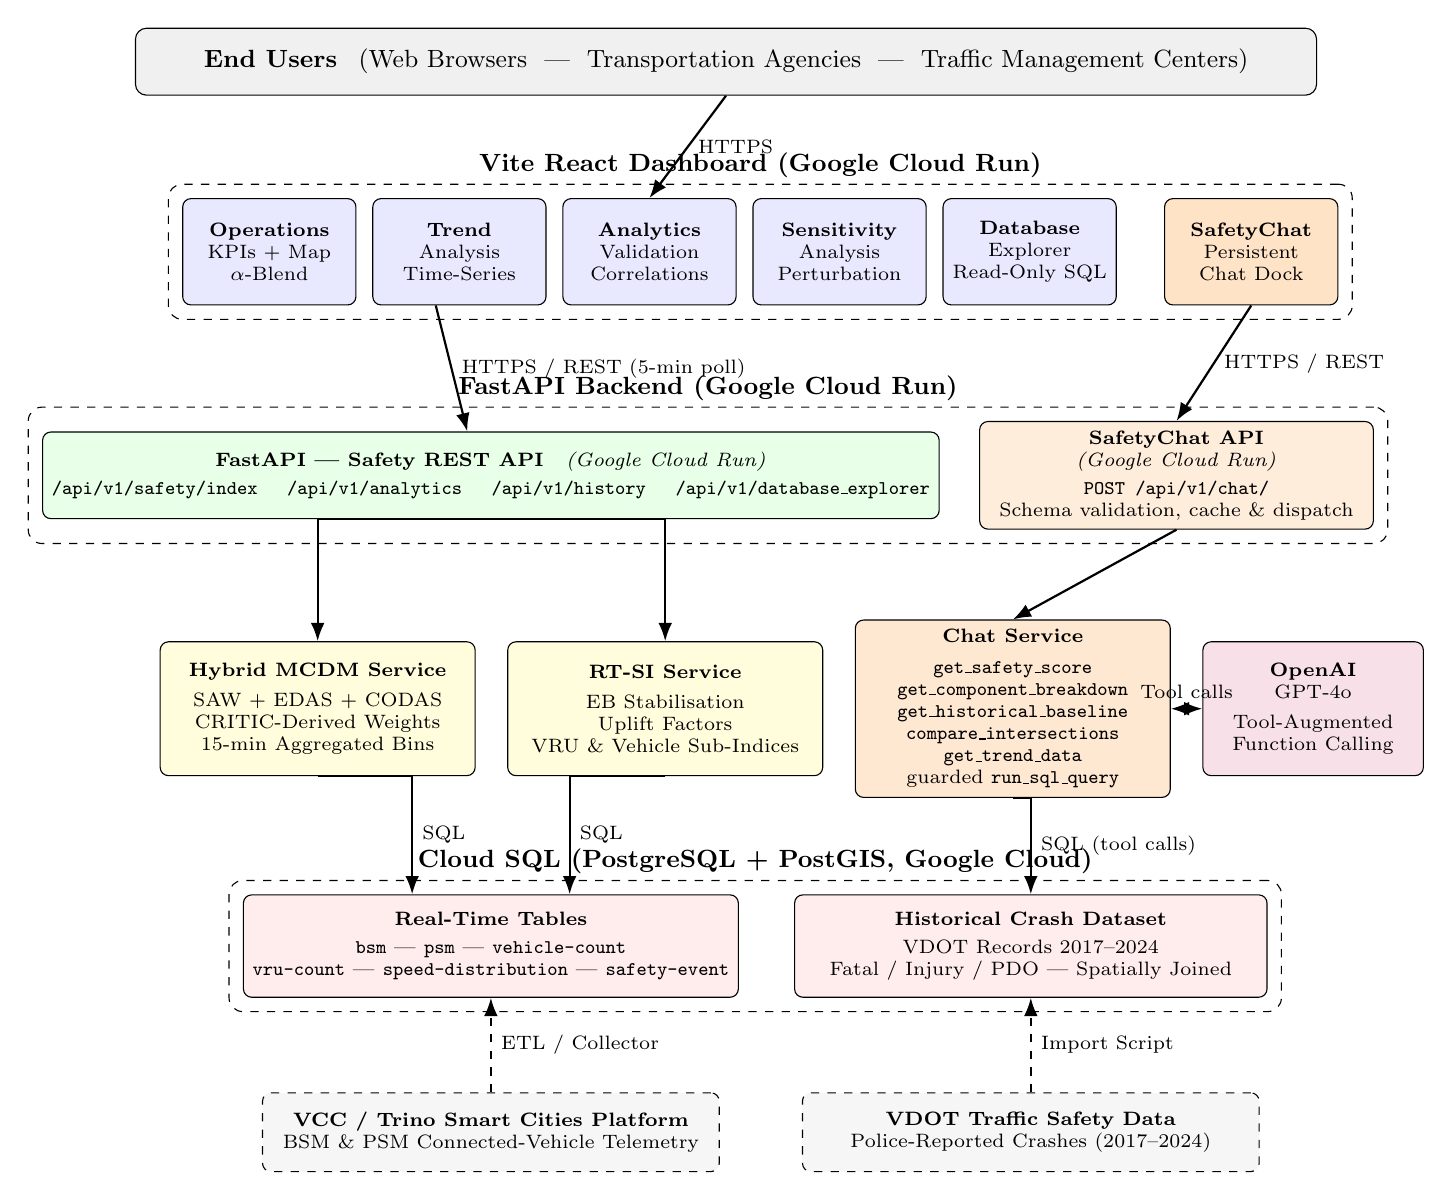
\begin{tikzpicture}[
    >=Latex,
    font=\small,
    % ── node styles ──────────────────────────────────────────
    user/.style    ={rectangle, draw, rounded corners=4pt, fill=gray!12,
                     minimum width=15cm, minimum height=0.85cm, align=center},
    page/.style    ={rectangle, draw, rounded corners=3pt, fill=blue!9,
                     minimum width=2.2cm, minimum height=1.35cm,
                     align=center, font=\scriptsize},
    chatpage/.style={rectangle, draw, rounded corners=3pt, fill=orange!22,
                     minimum width=2.2cm, minimum height=1.35cm,
                     align=center, font=\scriptsize},
    api/.style     ={rectangle, draw, rounded corners=3pt, fill=green!9,
                     minimum width=7.8cm, minimum height=1.1cm,
                     align=center, font=\scriptsize},
    chatapi/.style ={rectangle, draw, rounded corners=3pt, fill=orange!14,
                     minimum width=5.0cm, minimum height=1.1cm,
                     align=center, font=\scriptsize},
    svc/.style     ={rectangle, draw, rounded corners=3pt, fill=yellow!14,
                     minimum width=4.0cm, minimum height=1.7cm,
                     align=center, font=\scriptsize},
    chatsvc/.style ={rectangle, draw, rounded corners=3pt, fill=orange!18,
                     minimum width=4.0cm, minimum height=1.7cm,
                     align=center, font=\scriptsize},
    llm/.style     ={rectangle, draw, rounded corners=3pt, fill=purple!12,
                     minimum width=2.8cm, minimum height=1.7cm,
                     align=center, font=\scriptsize},
    dbtab/.style   ={rectangle, draw, rounded corners=3pt, fill=red!7,
                     minimum width=6.0cm, minimum height=1.3cm,
                     align=center, font=\scriptsize},
    ext/.style     ={rectangle, draw, dashed, rounded corners=3pt, fill=gray!7,
                     minimum width=5.8cm, minimum height=1.0cm,
                     align=center, font=\scriptsize},
    grpbox/.style  ={rectangle, draw, dashed, rounded corners=5pt, inner sep=5pt},
    arr/.style     ={->, thick, >=Latex},
    darr/.style    ={->, thick, dashed, >=Latex},
]

% ── TIER 0 : Users ────────────────────────────────────────────────────────────
\node[user] (user)
    {\textbf{End Users}
     \enspace(Web Browsers \ | \ Transportation Agencies \ | \
              Traffic Management Centers)};

% ── TIER 1 : Vite frontend dashboard panels ─────────────────────────────────
\node[page, below=1.3cm of user, xshift=-5.8cm] (p0)
    {\textbf{Operations}\\KPIs + Map\\$\alpha$-Blend};
\node[page, right=0.2cm of p0] (p1)
    {\textbf{Trend}\\Analysis\\Time-Series};
\node[page, right=0.2cm of p1] (p2)
    {\textbf{Analytics}\\Validation\\Correlations};
\node[page, right=0.2cm of p2] (p3)
    {\textbf{Sensitivity}\\Analysis\\Perturbation};
\node[page, right=0.2cm of p3] (p4)
    {\textbf{Database}\\Explorer\\Read-Only SQL};
\node[chatpage, right=0.6cm of p4] (p5)
    {\textbf{SafetyChat}\\Persistent\\Chat Dock};

\node[grpbox, fit=(p0)(p1)(p2)(p3)(p4)(p5),
      label={[font=\small\bfseries, fill=white, inner sep=2pt,
              rounded corners=2pt]above:{Vite React Dashboard (Google Cloud Run)}}]
      (fe_box) {};

% ── TIER 2 : Backend API layer ────────────────────────────────────────────────
% api_main placed so it roughly centres on analysis pages p0-p3
\node[api, below=1.6cm of p1, xshift=0.4cm] (api_main)
    {\textbf{FastAPI --- Safety REST API}\quad\textit{(Google Cloud Run)}\\[2pt]
     \texttt{/api/v1/safety/index} \quad
     \texttt{/api/v1/analytics} \quad
     \texttt{/api/v1/history} \quad
     \texttt{/api/v1/database\_explorer}};

\node[chatapi, right=0.5cm of api_main] (api_chat)
    {\textbf{SafetyChat API}\\
     \textit{(Google Cloud Run)}\\[2pt]
     \texttt{POST /api/v1/chat/}\\
     Schema validation, cache \& dispatch};

\node[grpbox, fit=(api_main)(api_chat),
      label={[font=\small\bfseries, fill=white, inner sep=2pt,
              rounded corners=2pt]above:{FastAPI Backend (Google Cloud Run)}}]
      (be_box) {};

% ── TIER 3 : Core services ────────────────────────────────────────────────────
\node[svc, below=1.55cm of api_main, xshift=-2.2cm] (mcdm)
    {\textbf{Hybrid MCDM Service}\\[3pt]
     SAW + EDAS + CODAS\\
     CRITIC-Derived Weights\\
     15-min Aggregated Bins};

\node[svc, right=0.4cm of mcdm] (rtsi)
    {\textbf{RT-SI Service}\\[3pt]
     EB Stabilisation\\
     Uplift Factors\\
     VRU \& Vehicle Sub-Indices};

\node[chatsvc, right=0.4cm of rtsi] (chatsvc)
    {\textbf{Chat Service}\\[3pt]
     \texttt{get\_safety\_score}\\
     \texttt{get\_component\_breakdown}\\
     \texttt{get\_historical\_baseline}\\
     \texttt{compare\_intersections}\\
     \texttt{get\_trend\_data}\\
     guarded \texttt{run\_sql\_query}};

\node[llm, right=0.4cm of chatsvc] (llm)
    {\textbf{OpenAI}\\GPT-4o\\[3pt]
     Tool-Augmented\\Function Calling};

% ── TIER 4 : Database ─────────────────────────────────────────────────────────
% db_rt centred roughly under mcdm+rtsi; db_crash under chatsvc
\node[dbtab, below=1.5cm of mcdm, xshift=2.2cm] (db_rt)
    {\textbf{Real-Time Tables}\\[2pt]
     \texttt{bsm} | \texttt{psm} | \texttt{vehicle-count}\\
     \texttt{vru-count} | \texttt{speed-distribution} | \texttt{safety-event}};

\node[dbtab, right=0.7cm of db_rt] (db_crash)
    {\textbf{Historical Crash Dataset}\\[2pt]
     VDOT Records 2017--2024\\
     Fatal / Injury / PDO --- Spatially Joined};

\node[grpbox, fit=(db_rt)(db_crash),
      label={[font=\small\bfseries, fill=white, inner sep=2pt,
              rounded corners=2pt]above:{Cloud SQL (PostgreSQL + PostGIS, Google Cloud)}}]
      (db_box) {};

% ── TIER 5 : External data sources ───────────────────────────────────────────
\node[ext, below=1.2cm of db_rt] (ext_vcc)
    {\textbf{VCC / Trino Smart Cities Platform}\\
     BSM \& PSM Connected-Vehicle Telemetry};

\node[ext, below=1.2cm of db_crash] (ext_vdot)
    {\textbf{VDOT Traffic Safety Data}\\
     Police-Reported Crashes (2017--2024)};

% ── ARROWS ────────────────────────────────────────────────────────────────────

% Users → Frontend (route to p2 node, centre of the analysis pages row)
\draw[arr] (user.south) -- node[right, font=\scriptsize]{HTTPS}
    (p2.north);

% Frontend analysis pages → Safety API (route straight into api_main)
\draw[arr] ([xshift=-0.3cm]p1.south) --
    node[right, font=\scriptsize]{HTTPS / REST (5-min poll)}
    ([xshift=-0.3cm]api_main.north);

% SafetyChat page → Chat API
\draw[arr] (p5.south) -- node[right, font=\scriptsize]{HTTPS / REST}
    (api_chat.north);

% Safety API → MCDM & RT-SI services
\draw[arr] (api_main.south) -| (mcdm.north);
\draw[arr] (api_main.south) -| (rtsi.north);

% Chat API → Chat Service
\draw[arr] (api_chat.south) -- (chatsvc.north);

% Chat Service <-> OpenAI (bidirectional)
\draw[<->, thick] (chatsvc.east) --
    node[above, font=\scriptsize]{Tool calls}
    (llm.west);

% MCDM → Real-Time DB
\draw[arr] (mcdm.south) -|
    node[pos=0.75, right, font=\scriptsize]{SQL}
    ([xshift=-1.0cm]db_rt.north);

% RT-SI → Historical DB
\draw[arr] (rtsi.south) -|
    node[pos=0.75, right, font=\scriptsize]{SQL}
    ([xshift=1.0cm]db_rt.north);

% Chat Service → Historical DB (LLM tool queries)
\draw[arr] (chatsvc.south) -|
    node[pos=0.75, right, font=\scriptsize]{SQL (tool calls)}
    (db_crash.north);

% External sources → DB (ETL ingestion, dashed)
\draw[darr] (ext_vcc.north) --
    node[right, font=\scriptsize]{ETL / Collector}
    (db_rt.south);
\draw[darr] (ext_vdot.north) --
    node[right, font=\scriptsize]{Import Script}
    (db_crash.south);

\end{tikzpicture}
 inside a figure* environment
% ============================================================
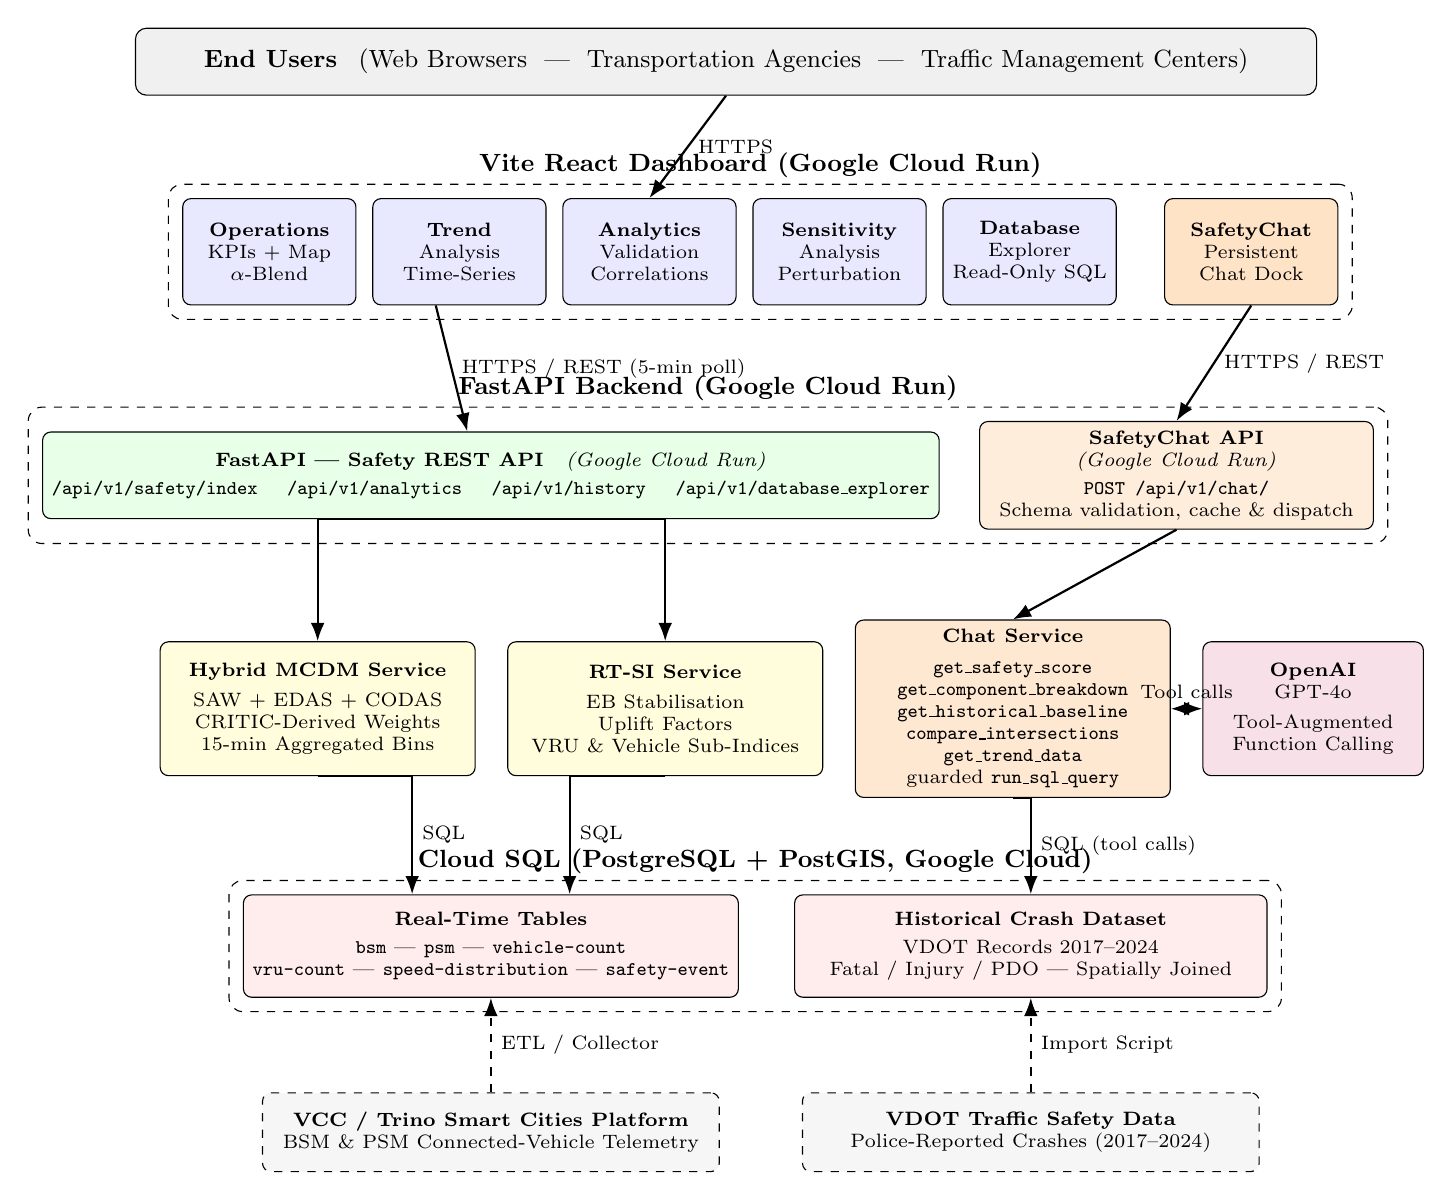
\begin{tikzpicture}[
    >=Latex,
    font=\small,
    % ── node styles ──────────────────────────────────────────
    user/.style    ={rectangle, draw, rounded corners=4pt, fill=gray!12,
                     minimum width=15cm, minimum height=0.85cm, align=center},
    page/.style    ={rectangle, draw, rounded corners=3pt, fill=blue!9,
                     minimum width=2.2cm, minimum height=1.35cm,
                     align=center, font=\scriptsize},
    chatpage/.style={rectangle, draw, rounded corners=3pt, fill=orange!22,
                     minimum width=2.2cm, minimum height=1.35cm,
                     align=center, font=\scriptsize},
    api/.style     ={rectangle, draw, rounded corners=3pt, fill=green!9,
                     minimum width=7.8cm, minimum height=1.1cm,
                     align=center, font=\scriptsize},
    chatapi/.style ={rectangle, draw, rounded corners=3pt, fill=orange!14,
                     minimum width=5.0cm, minimum height=1.1cm,
                     align=center, font=\scriptsize},
    svc/.style     ={rectangle, draw, rounded corners=3pt, fill=yellow!14,
                     minimum width=4.0cm, minimum height=1.7cm,
                     align=center, font=\scriptsize},
    chatsvc/.style ={rectangle, draw, rounded corners=3pt, fill=orange!18,
                     minimum width=4.0cm, minimum height=1.7cm,
                     align=center, font=\scriptsize},
    llm/.style     ={rectangle, draw, rounded corners=3pt, fill=purple!12,
                     minimum width=2.8cm, minimum height=1.7cm,
                     align=center, font=\scriptsize},
    dbtab/.style   ={rectangle, draw, rounded corners=3pt, fill=red!7,
                     minimum width=6.0cm, minimum height=1.3cm,
                     align=center, font=\scriptsize},
    ext/.style     ={rectangle, draw, dashed, rounded corners=3pt, fill=gray!7,
                     minimum width=5.8cm, minimum height=1.0cm,
                     align=center, font=\scriptsize},
    grpbox/.style  ={rectangle, draw, dashed, rounded corners=5pt, inner sep=5pt},
    arr/.style     ={->, thick, >=Latex},
    darr/.style    ={->, thick, dashed, >=Latex},
]

% ── TIER 0 : Users ────────────────────────────────────────────────────────────
\node[user] (user)
    {\textbf{End Users}
     \enspace(Web Browsers \ | \ Transportation Agencies \ | \
              Traffic Management Centers)};

% ── TIER 1 : Vite frontend dashboard panels ─────────────────────────────────
\node[page, below=1.3cm of user, xshift=-5.8cm] (p0)
    {\textbf{Operations}\\KPIs + Map\\$\alpha$-Blend};
\node[page, right=0.2cm of p0] (p1)
    {\textbf{Trend}\\Analysis\\Time-Series};
\node[page, right=0.2cm of p1] (p2)
    {\textbf{Analytics}\\Validation\\Correlations};
\node[page, right=0.2cm of p2] (p3)
    {\textbf{Sensitivity}\\Analysis\\Perturbation};
\node[page, right=0.2cm of p3] (p4)
    {\textbf{Database}\\Explorer\\Read-Only SQL};
\node[chatpage, right=0.6cm of p4] (p5)
    {\textbf{SafetyChat}\\Persistent\\Chat Dock};

\node[grpbox, fit=(p0)(p1)(p2)(p3)(p4)(p5),
      label={[font=\small\bfseries, fill=white, inner sep=2pt,
              rounded corners=2pt]above:{Vite React Dashboard (Google Cloud Run)}}]
      (fe_box) {};

% ── TIER 2 : Backend API layer ────────────────────────────────────────────────
% api_main placed so it roughly centres on analysis pages p0-p3
\node[api, below=1.6cm of p1, xshift=0.4cm] (api_main)
    {\textbf{FastAPI --- Safety REST API}\quad\textit{(Google Cloud Run)}\\[2pt]
     \texttt{/api/v1/safety/index} \quad
     \texttt{/api/v1/analytics} \quad
     \texttt{/api/v1/history} \quad
     \texttt{/api/v1/database\_explorer}};

\node[chatapi, right=0.5cm of api_main] (api_chat)
    {\textbf{SafetyChat API}\\
     \textit{(Google Cloud Run)}\\[2pt]
     \texttt{POST /api/v1/chat/}\\
     Schema validation, cache \& dispatch};

\node[grpbox, fit=(api_main)(api_chat),
      label={[font=\small\bfseries, fill=white, inner sep=2pt,
              rounded corners=2pt]above:{FastAPI Backend (Google Cloud Run)}}]
      (be_box) {};

% ── TIER 3 : Core services ────────────────────────────────────────────────────
\node[svc, below=1.55cm of api_main, xshift=-2.2cm] (mcdm)
    {\textbf{Hybrid MCDM Service}\\[3pt]
     SAW + EDAS + CODAS\\
     CRITIC-Derived Weights\\
     15-min Aggregated Bins};

\node[svc, right=0.4cm of mcdm] (rtsi)
    {\textbf{RT-SI Service}\\[3pt]
     EB Stabilisation\\
     Uplift Factors\\
     VRU \& Vehicle Sub-Indices};

\node[chatsvc, right=0.4cm of rtsi] (chatsvc)
    {\textbf{Chat Service}\\[3pt]
     \texttt{get\_safety\_score}\\
     \texttt{get\_component\_breakdown}\\
     \texttt{get\_historical\_baseline}\\
     \texttt{compare\_intersections}\\
     \texttt{get\_trend\_data}\\
     guarded \texttt{run\_sql\_query}};

\node[llm, right=0.4cm of chatsvc] (llm)
    {\textbf{OpenAI}\\GPT-4o\\[3pt]
     Tool-Augmented\\Function Calling};

% ── TIER 4 : Database ─────────────────────────────────────────────────────────
% db_rt centred roughly under mcdm+rtsi; db_crash under chatsvc
\node[dbtab, below=1.5cm of mcdm, xshift=2.2cm] (db_rt)
    {\textbf{Real-Time Tables}\\[2pt]
     \texttt{bsm} | \texttt{psm} | \texttt{vehicle-count}\\
     \texttt{vru-count} | \texttt{speed-distribution} | \texttt{safety-event}};

\node[dbtab, right=0.7cm of db_rt] (db_crash)
    {\textbf{Historical Crash Dataset}\\[2pt]
     VDOT Records 2017--2024\\
     Fatal / Injury / PDO --- Spatially Joined};

\node[grpbox, fit=(db_rt)(db_crash),
      label={[font=\small\bfseries, fill=white, inner sep=2pt,
              rounded corners=2pt]above:{Cloud SQL (PostgreSQL + PostGIS, Google Cloud)}}]
      (db_box) {};

% ── TIER 5 : External data sources ───────────────────────────────────────────
\node[ext, below=1.2cm of db_rt] (ext_vcc)
    {\textbf{VCC / Trino Smart Cities Platform}\\
     BSM \& PSM Connected-Vehicle Telemetry};

\node[ext, below=1.2cm of db_crash] (ext_vdot)
    {\textbf{VDOT Traffic Safety Data}\\
     Police-Reported Crashes (2017--2024)};

% ── ARROWS ────────────────────────────────────────────────────────────────────

% Users → Frontend (route to p2 node, centre of the analysis pages row)
\draw[arr] (user.south) -- node[right, font=\scriptsize]{HTTPS}
    (p2.north);

% Frontend analysis pages → Safety API (route straight into api_main)
\draw[arr] ([xshift=-0.3cm]p1.south) --
    node[right, font=\scriptsize]{HTTPS / REST (5-min poll)}
    ([xshift=-0.3cm]api_main.north);

% SafetyChat page → Chat API
\draw[arr] (p5.south) -- node[right, font=\scriptsize]{HTTPS / REST}
    (api_chat.north);

% Safety API → MCDM & RT-SI services
\draw[arr] (api_main.south) -| (mcdm.north);
\draw[arr] (api_main.south) -| (rtsi.north);

% Chat API → Chat Service
\draw[arr] (api_chat.south) -- (chatsvc.north);

% Chat Service <-> OpenAI (bidirectional)
\draw[<->, thick] (chatsvc.east) --
    node[above, font=\scriptsize]{Tool calls}
    (llm.west);

% MCDM → Real-Time DB
\draw[arr] (mcdm.south) -|
    node[pos=0.75, right, font=\scriptsize]{SQL}
    ([xshift=-1.0cm]db_rt.north);

% RT-SI → Historical DB
\draw[arr] (rtsi.south) -|
    node[pos=0.75, right, font=\scriptsize]{SQL}
    ([xshift=1.0cm]db_rt.north);

% Chat Service → Historical DB (LLM tool queries)
\draw[arr] (chatsvc.south) -|
    node[pos=0.75, right, font=\scriptsize]{SQL (tool calls)}
    (db_crash.north);

% External sources → DB (ETL ingestion, dashed)
\draw[darr] (ext_vcc.north) --
    node[right, font=\scriptsize]{ETL / Collector}
    (db_rt.south);
\draw[darr] (ext_vdot.north) --
    node[right, font=\scriptsize]{Import Script}
    (db_crash.south);

\end{tikzpicture}
%
}
\caption{VTTSI cloud-native system architecture. The orange pathway (SafetyChat API,
         Chat Service, OpenAI GPT-4o) is the new contribution of this demo paper;
         the blue/green/yellow left pathway shows the existing safety-index pipeline.}
\label{fig:architecture}
\end{figure*}

The VTTSI backend (FastAPI, Google Cloud Run) computes two complementary safety indices
every 15 minutes from connected-vehicle telemetry streamed via the VTTI Trino system
and stored in Cloud SQL PostgreSQL.

\subsection{Real-Time Safety Index (RT--SI)}

RT--SI anchors intersection risk to a severity-weighted Empirical Bayes (EB) baseline
derived from 2017--2024 VDOT crash records.
The historical crash rate is:
\begin{equation}
r_i = \frac{\sum_{s}\, w_s\, C_{i,s}}{E_i},
\quad w_{\text{Fatal}}=10,\; w_{\text{Inj}}=3,\; w_{\text{PDO}}=1,
\end{equation}
where $C_{i,s}$ are crash counts by severity and $E_i$ is vehicle exposure.
The EB stabilized rate is:
\begin{equation}
\hat{r}^{\text{EB}}_{i,t}(\lambda) =
\frac{Y_{i,t} + \lambda\, r_0}{1 + \lambda},
\quad \lambda^\star = 10{,}000,
\end{equation}
where $r_0$ is the global mean rate across all site-bins (2017--2024) and
$\lambda^\star$ is chosen by minimizing Poisson log-loss on a 2025 hold-out set.
Real-time uplift factors---bounded to $[0,1]$---adjust this baseline for speed deficit
($F^{\text{spd}}$), speed variance ($F^{\text{var}}$), and VRU--vehicle conflict
exposure ($F^{\text{conf}}$):
\begin{equation}
U_{i,t} = 1 + \beta_1 F^{\text{spd}}_{i,t}
              + \beta_2 F^{\text{var}}_{i,t}
              + \beta_3 F^{\text{conf}}_{i,t}.
\end{equation}
VRU and vehicle sub-indices are multiplied by $U_{i,t}$ and the EB baseline,
combined with weights $\omega_{\text{vru}}$ and $\omega_{\text{veh}}$,
and min-max scaled to produce $\mathrm{SI}^{\text{RT}}\in[0,100]$.

\subsection{MCDM Safety Index}

A CRITIC-weighted multi-criteria pipeline \cite{Amraji2025CombinedSafetyIndex}
constructs a decision matrix over five real-time criteria
(vehicle count, VRU count, average speed, speed variance, incident count)
for each intersection--time-bin pair.
CRITIC criterion weights are derived from normalized standard deviations and
inter-criterion Pearson correlations, recomputed every 24 hours.
Three MCDM scoring methods---SAW, EDAS, and CODAS---are each computed and scaled
to $[0,100]$; a second-pass CRITIC aggregation yields the hybrid index
$\mathrm{SI}^{\text{MCDM}}\in[0,100]$ (higher = higher risk).

\subsection{Blended Final Index}

\begin{equation}
\mathrm{SI}^{\text{Final}}_{i,t} =
\alpha\,\mathrm{SI}^{\text{RT}}_{i,t} +
(1-\alpha)\,\mathrm{SI}^{\text{MCDM}}_{i,t},
\quad \alpha = 0.7\text{ (default)}.
\label{eq:blend}
\end{equation}

Scores map to risk levels: 0--40 = low, 41--70 = moderate, 71--100 = high.
The $\alpha$ parameter is user-adjustable to shift emphasis between historical risk
and instantaneous anomaly detection.

\subsection{Geospatial Data Foundation}

Each intersection is registered with a centroid $(lat_i, lon_i)$ and an
axis-aligned bounding box $B_i$ ($\delta\!\approx\!0.001^{\circ}$, $\approx$111\,m).
VDOT crash records are assigned to intersections at import time via a PostGIS
\texttt{ST\_Within} predicate; overlaps are resolved by minimum Haversine distance.
This one-time spatial join materialises the per-site counts $C_{i,s}$ (Eq.~(1))
as a static lookup table.
The Streamlit Dashboard polls \texttt{/api/v1/safety/index} every five minutes and
recolors each \texttt{folium.CircleMarker}---\textcolor{green!60!black}{green}
($\mathrm{SI}<60$), \textcolor{orange!80!black}{amber} (60--75),
\textcolor{red}{red} ($>75$)---with radius proportional to traffic volume,
giving operators a dual spatial encoding of risk and exposure
(Figure~\ref{fig:demo-screenshots}a).

% ─────────────────────────────────────────────────────────
\section{SafetyChat: LLM-Powered Explanation Module}
\label{sec:safetychat}

VTTSI already answers \emph{what} the score is; SafetyChat answers \emph{why} and
\emph{what to do}.
GPT-4o is equipped with typed function calls \cite{openai_functioncalling} that map
to VTTSI REST endpoints, grounding every claim in live data.
An agentic loop (up to six iterations) enables chained calls---e.g., ranking all
intersections then drilling into the top site's breakdown.
The six tools are:
(1)~\texttt{get\_safety\_score} --- RT--SI, MCDM, and blended scores with uplift
factors; optional \texttt{target\_time} for historical queries;
(2)~\texttt{get\_component\_breakdown} --- CRITIC-weighted criteria for a 15-min bin;
(3)~\texttt{get\_historical\_baseline} --- EB prior and 7-year crash severity breakdown;
(4)~\texttt{compare\_intersections} --- ranks all sites by any index component;
(5)~\texttt{get\_trend\_data} --- 7--30 day MCDM trend with sampled snapshots;
(6)~\texttt{run\_sql\_query} --- read-only ad-hoc SQL, write-guarded.

Table~\ref{tbl:comparison} positions VTTSI-Chat against related systems.

\begin{table}[t]
\centering
\caption{VTTSI-Chat vs.\ Related Systems}
\label{tbl:comparison}
\small
\setlength{\tabcolsep}{4pt}
\begin{tabularx}{\columnwidth}{@{}l c c c c@{}}
\toprule
\textbf{System} &
\textbf{\shortstack{Hybrid\\Index}} &
\textbf{\shortstack{Real-Time\\Telemetry}} &
\textbf{\shortstack{LLM\\Interface}} &
\textbf{\shortstack{Causal\\Narrative}} \\
\midrule
Google / Apple Maps              & \xmark & \cmark & \xmark & \xmark \\
Waycare / ATSPM                  & \xmark & \cmark & \xmark & \xmark \\
TrafficGPT \cite{trafficgpt2023} & \xmark & \cmark & \cmark & \xmark \\
LLMLight \cite{llmlight2024}     & \xmark & \cmark & \cmark & \xmark \\
GPT-Driver \cite{gptdriver2023}  & \xmark & \cmark & \cmark & \xmark \\
\textbf{VTTSI-Chat (ours)}       & \cmark & \cmark & \cmark & \cmark \\
\bottomrule
\end{tabularx}
\end{table}

% ─────────────────────────────────────────────────────────
\section{Demonstration}
\label{sec:demo}

The live demo runs against the production VTTSI deployment, monitoring 18
intersections in Falls Church, VA. Four use cases are demonstrated.

\subsection{UC1: TMC Operator Morning Briefing}
\textit{Query:} \emph{``Give me a morning safety briefing for all intersections.''}
SafetyChat chains \texttt{compare\_intersections} and \texttt{get\_component\_breakdown}
for the two highest-ranked sites, delivering a situational-awareness narrative
identifying peak-risk windows and dominant criteria (e.g., speed variance, VRU counts)
in under five seconds.

\subsection{UC2: Causal Safety Explanation for Planners}
\textit{Query:} \emph{``Why did E.~Broad--N.~Washington score above 70 yesterday at 5\,PM?''}
SafetyChat queries \texttt{get\_safety\_score} and \texttt{get\_component\_breakdown}
at the historical time-bin, identifies criteria in the 90th percentile, and traces
the elevated score to concurrent peak vehicle volume and incident activity.

\subsection{UC3: Emergency Responder Routing}
\textit{Query:} \emph{``Which of Glebe--Potomac or Birch--W.~Broad has lower current risk?''}
SafetyChat compares live RT--SI, MCDM, and blended indices for both intersections and
recommends the lower-risk route with reasoning grounded in VRU counts and speed variance.

\subsection{UC4: Public Stakeholder Trend Engagement}
\textit{Query:} \emph{``Is the Glebe--Potomac intersection getting safer over time?''}
SafetyChat calls \texttt{get\_trend\_data} (30-day window) and translates mean/max/min
MCDM scores into plain-language risk levels with a trend direction indicator.

\begin{figure*}[t]
\centering
\begin{minipage}[t]{0.48\textwidth}
  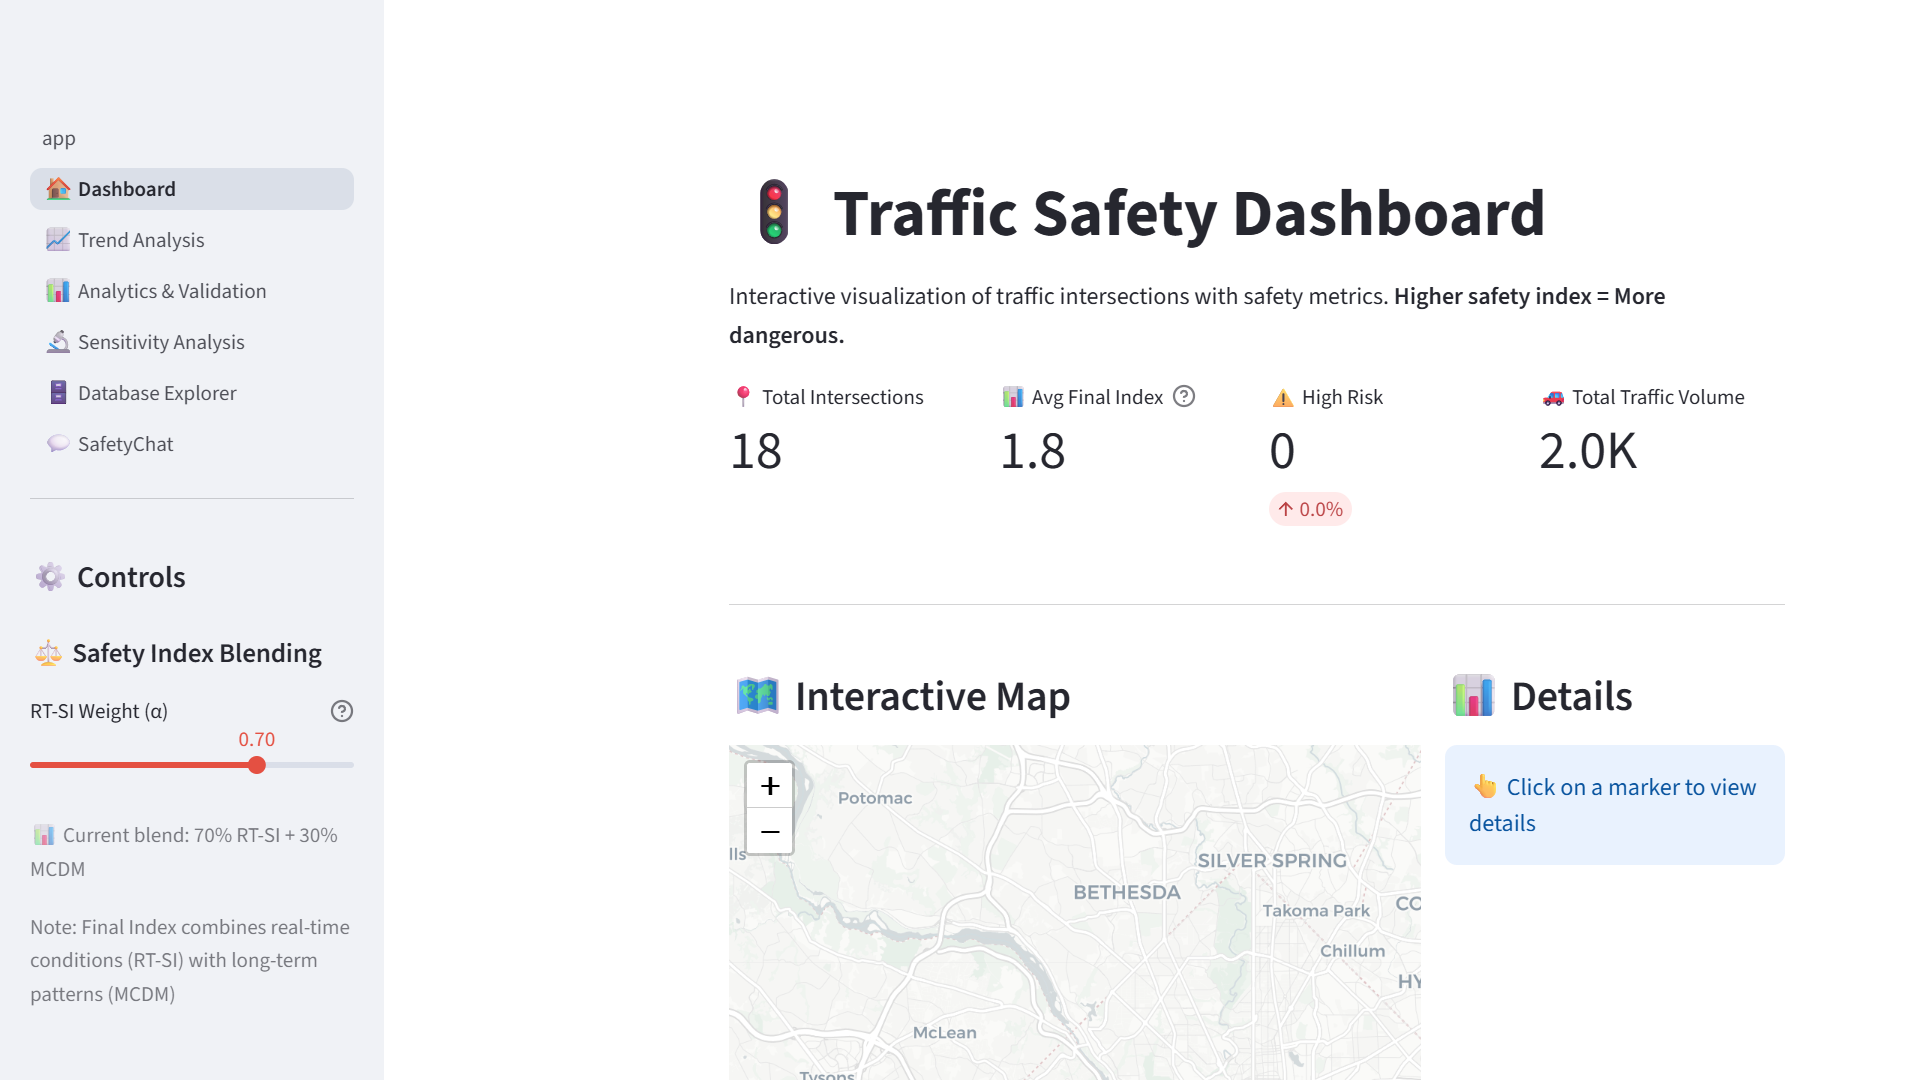
\includegraphics[height=1.6in,keepaspectratio,width=\textwidth]{screenshot_dashboard.png}\\[-0.2ex]
  {\small\textit{(a) Dashboard: interactive map with 18 monitored intersections (Falls Church, VA),
  real-time KPI cards (Avg Index 1.8, 0 High-Risk sites, 2.0\,K traffic volume).}}
\end{minipage}\hfill
\begin{minipage}[t]{0.48\textwidth}
  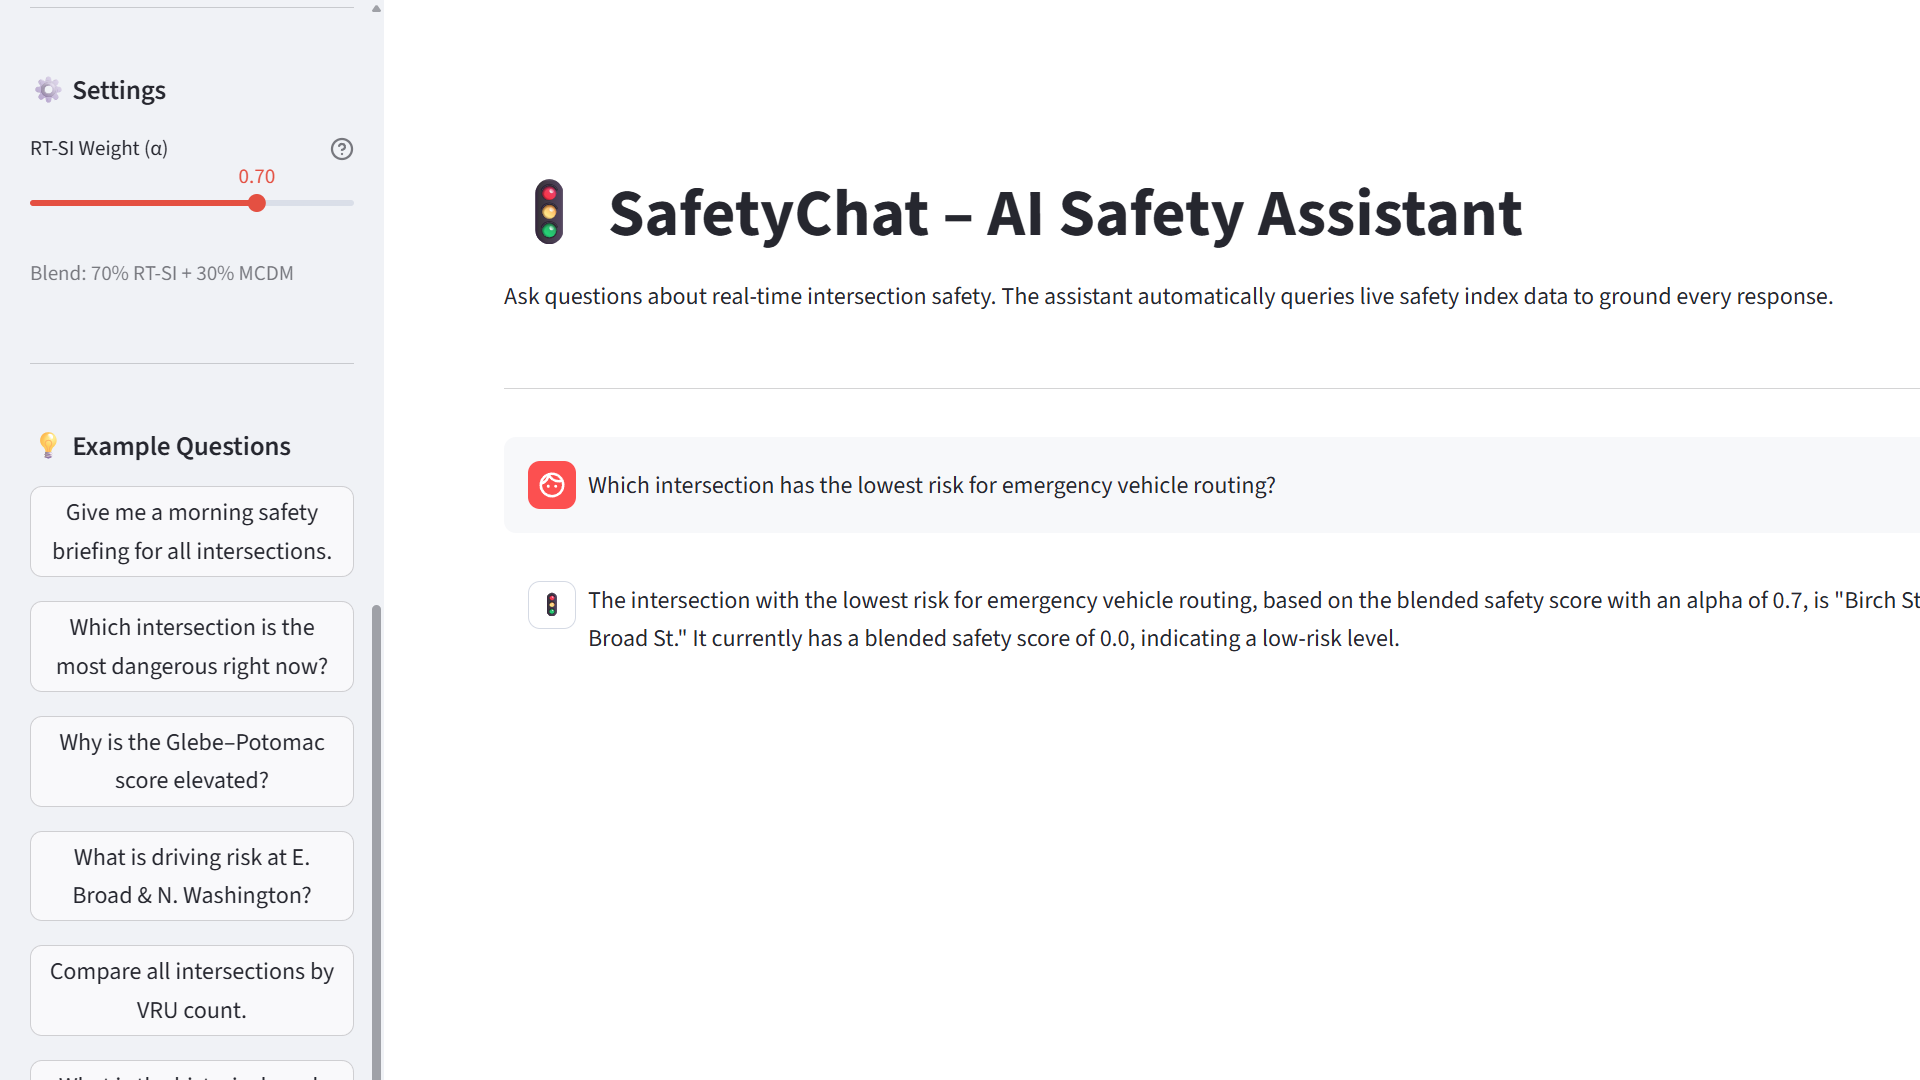
\includegraphics[height=1.6in,keepaspectratio,width=\textwidth]{screenshot_safetychat_uc3_clean.png}\\[-0.2ex]
  {\small\textit{(b) SafetyChat (UC3): emergency routing query---GPT-4o calls
  \texttt{compare\_intersections} and returns Birch \& W.\,Broad as the safest
  crossing (blended score 0.0) for immediate vehicle dispatch.}}
\end{minipage}
\caption{Live VTTSI-Chat demonstration: (a)~geospatial dashboard providing
  system-wide situational awareness; (b)~SafetyChat natural-language response
  grounding an emergency routing recommendation in live blended safety indices.}
\label{fig:demo-screenshots}
\end{figure*}

\begin{table}[t]
\centering
\caption{Summary of Demonstration Use Cases}
\label{tbl:usecases}
\small
\begin{tabularx}{\columnwidth}{@{}l X l@{}}
\toprule
\textbf{Use Case} & \textbf{Key Tool Calls} & \textbf{User} \\
\midrule
Morning briefing     & compare + breakdown        & TMC Operator \\
Causal explanation   & score(t) + breakdown(t)    & Planner \\
Responder routing    & score $\times$ 2           & Dispatcher \\
Trend engagement     & get\_trend\_data(30d)      & Official/Public \\
\bottomrule
\end{tabularx}
\end{table}

% ─────────────────────────────────────────────────────────
\section{Related Work}
\label{sec:related}

VTTSI's scoring builds on EB-stabilized crash models
\cite{persaud2007,montella2020systemic}, MCDM-based indices
\cite{Amraji2025CombinedSafetyIndex,asadamraji2025combined}, and surrogate safety
indicators \cite{schultz2025_surrogate,gettman2003ssam}.
In the LLM domain, TrafficGPT \cite{trafficgpt2023}, LLMLight \cite{llmlight2024},
and GPT-Driver/DriveVLM \cite{gptdriver2023,drivevlm2024} address flow analysis,
signal control, and AV planning respectively---none provide a safety-index explanation
interface for infrastructure operators.

% ─────────────────────────────────────────────────────────
\section{Conclusion}
\label{sec:conclusion}

VTTSI-Chat closes the gap between quantitative safety scoring and actionable
situational awareness by grounding all LLM outputs in six typed API tool calls,
delivering causally grounded safety narratives to TMC operators, planners, and
emergency responders through natural language dialogue.
The spatially-joined crash baseline, bounding-box intersection registry, and live
15-minute telemetry together form the \emph{foundational geospatial layer} for future
work integrating the Agentic Traffic Safety Knowledge Graph (TS--KG)---enabling the
LLM to reason over intersection geometry, conflict topology, and causal trajectory
motifs.

\section*{Acknowledgment}
The VTTSI system was developed in collaboration with the Virginia Tech Transportation
Institute (VTTI).
Generative AI tools, including OpenAI ChatGPT (GPT-4o) and Anthropic Claude, were
utilized to assist in generating portions of this work, including manuscript text,
LaTeX formatting, and code snippets.
All AI-generated content was reviewed, verified, and edited by the authors, who take
full responsibility for the accuracy and integrity of the submitted manuscript.

\printbibliography

\end{document}
